\documentclass[tikz,border=3pt]{standalone}
\usetikzlibrary{calc}
\begin{document}
%\tikz \draw (-1.5, 0) -- (1.5, 1);
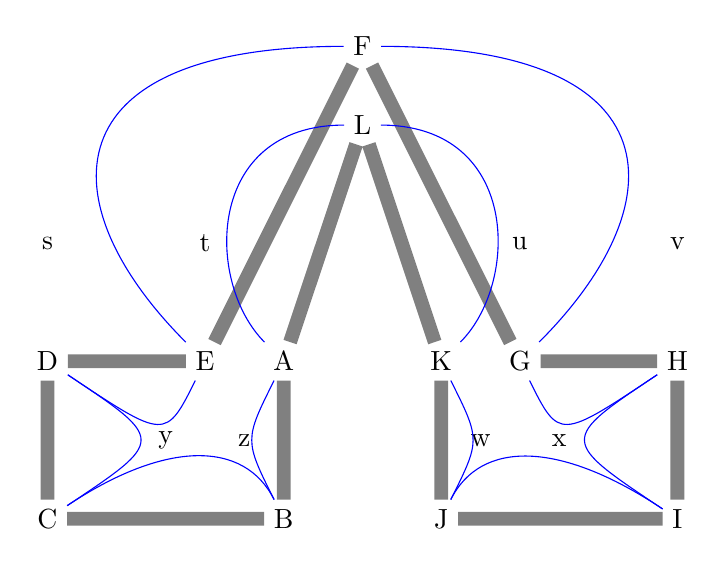
\begin{tikzpicture}
  \node (a) at (3,3) {A};
  \node (b) at (3,1) {B};
  \node (c) at (0,1) {C};
  \node (d) at (0,3) {D};
  \node (e) at (2,3) {E};
  \node (f) at (4,7) {F};
  \node (g) at (6,3) {G};
  \node (h) at (8,3) {H};
  \node (i) at (8,1) {I};
  \node (j) at (5,1) {J};
  \node (k) at (5,3) {K};
  \node (l) at (4,6) {L};
  \node (z) at (2.5,2) {z};
  \node (y) at (1.5,2) {y};
  \node (x) at (6.5,2) {x};
  \node (w) at (5.5,2) {w};
  \node (v) at (8,4.5) {v};
  \node (u) at (6,4.5) {u};
  \node (t) at (2,4.5) {t};
  \node (s) at (0,4.5) {s};
  
  % backbone controls
  \draw[line width=5pt, color=gray] (a) -- (b) -- (c) -- (d) -- (e) -- (f)
  -- (g) -- (h) -- (i) -- (j) -- (k) -- (l) -- (a);
  % left leg
  \draw[blue] (a) .. controls (z) .. (b);
  \draw[blue] (b) .. controls (z) and (y) .. (c);
  \draw[blue] (c) .. controls (y) .. (d);
  \draw[blue] (d) .. controls (y) .. (e);
  % top arch
  \draw[blue] (e) .. controls (0,5) and (0,7) .. (f);
    \draw[blue] (g) .. controls (8,5) and (8,7) .. (f);
  %\draw[blue] (k) .. controls ($(u) + (0,1)$) and ($(u) - (0,1)$) .. (l);
  \draw[blue] (k) .. controls (6,4) and (6,6) .. (l);
  \draw[blue] (a) .. controls (2,4) and (2,6) .. (l);
  % right leg
  \draw[blue] (g) .. controls (x) .. (h);
  \draw[blue] (h) .. controls (x) .. (i);
  \draw[blue] (i) .. controls (x) and (w) .. (j);
  \draw[blue] (j) .. controls (w) .. (k);

  
  %\draw[line width=10pt] (0,0) .. controls (1,1) .. (4,0) .. controls (5,0) and (5,1) .. (4,1);
\end{tikzpicture}


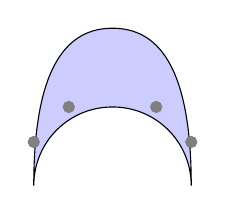
\begin{tikzpicture}
    \draw[fill=blue!20] (-1,0) .. controls (-1,0.555) and (-0.555,1) .. (0,1)
    .. controls (0.555,1) and (1,0.555) .. (1,0) .. controls (1, 1.555) and (0.555, 2) .. (0, 2)
    .. controls (-0.555, 2) and (-1, 1.555) .. (-1, 0) -- cycle;

    \filldraw[gray] (-1,0.555) circle [radius=2pt]
    (-0.555,1) circle [radius=2pt]
    (0.555, 1) circle [radius=2pt]
    (1,0.555) circle [radius=2pt];
\end{tikzpicture}

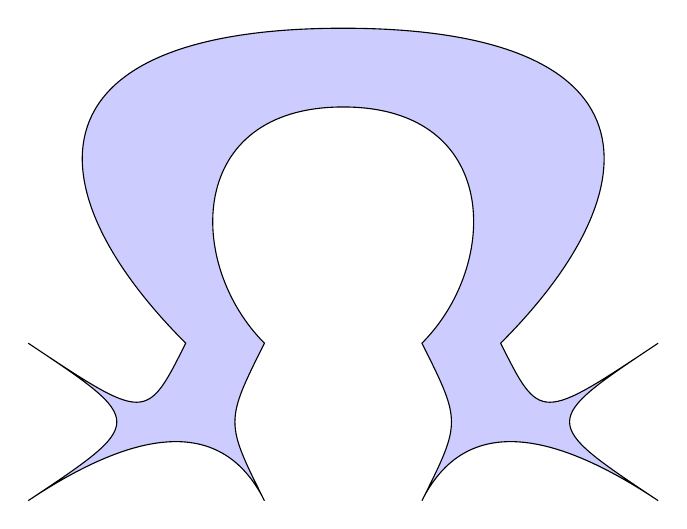
\begin{tikzpicture}
  \coordinate (a) at (3,3) {};
  \coordinate (b) at (3,1) {};
  \coordinate (c) at (0,1) {};
  \coordinate (d) at (0,3) {};
  \coordinate (e) at (2,3) {};
  \coordinate (f) at (4,7) {};
  \coordinate (g) at (6,3) {};
  \coordinate (h) at (8,3) {};
  \coordinate (i) at (8,1) {};
  \coordinate (j) at (5,1) {};
  \coordinate (k) at (5,3) {};
  \coordinate (l) at (4,6) {};
  \coordinate (z) at (2.5,2) {};
  \coordinate (y) at (1.5,2) {};
  \coordinate (x) at (6.5,2) {};
  \coordinate (w) at (5.5,2) {};
  \coordinate (v) at (8,4.5) {};
  \coordinate (u) at (6,4.5) {};
  \coordinate (t) at (2,4.5) {};
  \coordinate (s) at (0,4.5) {};

  \draw[fill=blue!20] (a) .. controls (z) .. (b)
  .. controls (z) and (y) .. (c)
  .. controls (y) .. (d)
  .. controls (y) .. (e)
  .. controls (0,5) and (0,7) .. (f)
  .. controls (8,7) and (8,5) .. (g)
  .. controls (x) .. (h)
  .. controls (x) .. (i)
  .. controls (x) and (w) .. (j)
  .. controls (w) .. (k)
  .. controls (6,4) and (6,6) .. (l)
  .. controls (2,6) and (2,4) .. (a) -- cycle;
\end{tikzpicture}


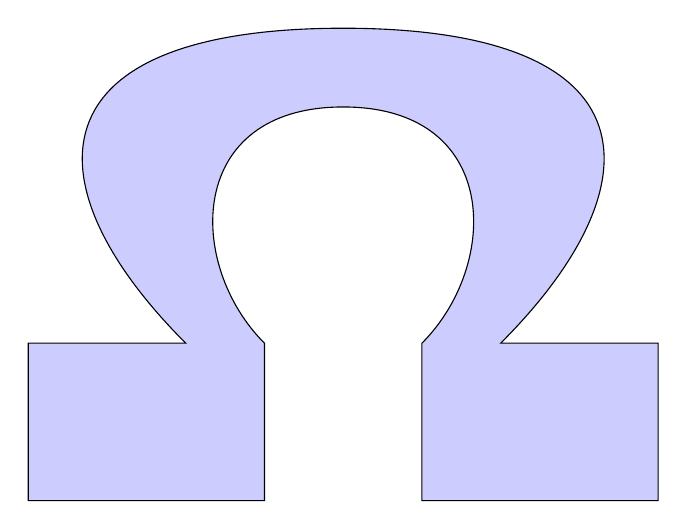
\begin{tikzpicture}[relative=false]
  \coordinate (a) at (3,3) {};
  \coordinate (b) at (3,1) {};
  \coordinate (c) at (0,1) {};
  \coordinate (d) at (0,3) {};
  \coordinate (e) at (2,3) {};
  \coordinate (f) at (4,7) {};
  \coordinate (g) at (6,3) {};
  \coordinate (h) at (8,3) {};
  \coordinate (i) at (8,1) {};
  \coordinate (j) at (5,1) {};
  \coordinate (k) at (5,3) {};
  \coordinate (l) at (4,6) {};
  \coordinate (z) at (2.5,2) {};
  \coordinate (y) at (1.5,2) {};
  \coordinate (x) at (6.5,2) {};
  \coordinate (w) at (5.5,2) {};
  \coordinate (v) at (8,4.5) {};
  \coordinate (u) at (6,4.5) {};
  \coordinate (t) at (2,4.5) {};
  \coordinate (s) at (0,4.5) {};

  \draw[fill=blue!20] (a) to[out=270,in=90] (b)
  to[out=180,in=0] (c)
  to[out=90,in=270] (d)
  to[out=0,in=180] (e)
  .. controls (0,5) and (0,7) .. (f)
  .. controls (8,7) and (8,5) .. (g)
  to[out=0,in=180] (h)
  to[out=270,in=90] (i)
  to[out=180,in=0] (j)
  to[out=90, in=270] (k)
  .. controls (6,4) and (6,6) .. (l)
  .. controls (2,6) and (2,4) .. (a) -- cycle;
\end{tikzpicture}

\begin{tikzpicture}[out=180,in=135]
\draw (0,0) to (1,0)
to (2,1)
to (2,2);
\end{tikzpicture}



\begin{tikzpicture}[line width=3pt,xscale=0.7,yscale=0.7,line cap=round, line join=round]
  \draw[fill=red] (-0.1, 0) coordinate (a) arc [start angle=-60, end angle=240,
  x radius=0.75cm, y radius=0.66cm] coordinate (b);
  \draw (0.66, 0) coordinate (c) arc [start angle=-30, end angle=210,
  x radius=1.3cm, y radius=1cm] coordinate (d);
  \draw (c) to[out=0,in=225] ++(0.66,0) to[out=-105,in=105] ++(0,-0.66) to[out=165,in=15] ++(-1.5,0.1) to[out=75,in=-75] (a);
  \draw (d) to[out=180,in=-45] ++(-0.66,0) to[out=-75,in=75] ++(0,-0.66) to[out=15,in=165] ++(1.5,0.1) to[out=105,  in=-105] (b);

\end{tikzpicture}


\begin{tikzpicture}[line width=3pt,xscale=0.7,yscale=0.7,line cap=round, line join=round]
  \draw[fill=purple] (-0.1, 0) coordinate (a) arc [start angle=-60, end angle=240,
  x radius=0.75cm, y radius=0.66cm] coordinate (b) (0.66, 0) coordinate (c) arc [start angle=-30, end angle=210,
  x radius=1.3cm, y radius=1cm] coordinate (d) (c) to[out=0,in=225] ++(0.66,0) to[out=-105,in=105] ++(0,-0.66) to[out=165,in=15] ++(-1.5,0.1) to[out=75,in=-75] (a) (d) to[out=180,in=-45] ++(-0.66,0) to[out=-75,in=75] ++(0,-0.66) to[out=15,in=165] ++(1.5,0.1) to[out=105,  in=-105] (b);

\end{tikzpicture}




\begin{tikzpicture}
  % Use even odd rule to fill the outer arc minus the inner arc
  \path[fill=gray!30, even odd rule]
    % --- Outer arc (big ellipse) ---
    (0.66, 0) arc [
      start angle=-30, end angle=210,
      x radius=2cm, y radius=1.33cm
    ]
    -- cycle
    % --- Inner arc (smaller ellipse) ---
    (0, 0) arc [
      start angle=-45, end angle=225,
      x radius=1.5cm, y radius=1cm
    ]
    -- cycle;
\end{tikzpicture}



\begin{tikzpicture}[line width=3pt,xscale=0.6,yscale=0.7,line cap=round, line join=round]
\definecolor{bostonuniversityred}{rgb}{0.8, 0.0, 0.0}
  \coordinate (c) at (0.66,0);
  
  \path[
    fill=bostonuniversityred,            % Fill the interior in red
    draw=black]

    (c)
      arc [
        start angle=-30, end angle=210,
        x radius=1.3cm, y radius=1cm
      ] coordinate (d)

      to[out=180, in=-45] ++(-0.66,0)
      to[out=-75, in=75]  ++(0,-0.66)
      to[out=15,  in=165] ++(1.5,0.1)
      to[out=105, in=-105] coordinate (b) ++(0,0.5)

      arc [
        start angle=240, end angle=-60,
        x radius=0.75cm, y radius=0.66cm
      ] coordinate (a)

      to[out=-75,in=75] ++(0,-0.6)
      to[out=15, in=165] ++(1.33,0.1)
      to[out=105, in=-105] ++(0,0.66)
      to[out=225, in=0] (c) -- cycle;

\end{tikzpicture}



\end{document}

